\documentclass[uplatex,dvipdfmx]{jsarticle}

\usepackage[uplatex,deluxe]{otf} % UTF
\usepackage[noalphabet]{pxchfon} % must be after otf package
\usepackage{stix2} %欧文&数式フォント
\usepackage[fleqn,tbtags]{mathtools} % 数式関連 (w/ amsmath)
\usepackage{hira-stix} % ヒラギノフォント&STIX2 フォント代替定義(Warning回避)

\begin{document}

\title{仕様書} %システム名 仕様書 という形式にする
\author{24G1007 網中洲}
\date{2025年01月7日}
\maketitle
\section{概要}
このアプリケーションは,シンプルな掲示板(BBS)システムを実装しています.ユーザーは以下の操作を行うことができる.
\begin{enumerate}
  \setlength{\leftskip}{0pt}
  \item[(1)]投稿(名前,メッセージの送信).

  \item[(2)]投稿一覧の取得(リアルタイム更新).
  \item[(3)]投稿の検索(キーワード検索).
  
  \item[(4)]投稿の編集および削除.
  \item[(5)]投稿への「いいね」.
\end{enumerate}




\section{利用者向けの説明}
画面のレイアウトは,以下の図\ref{reiauto}のようになる.
「送信」ボタンを押すと,名前とメッセージが送信され,「投稿チェック」ボタンを押すと,投稿された名前とメッセージを閲覧できる.
さらに,投稿されたメッセージごとに「いいね」ボタン,「編集」ボタン,「削除」ボタンがある.
これらは,投稿されたメッセージの評価,編集,削除ができる.
また,上部に「検索」ボタンがある.これは,検索したいメッセージの一部を入力することで,見たいメッセージを検索できる.

\begin{figure}[H]
  \centering
      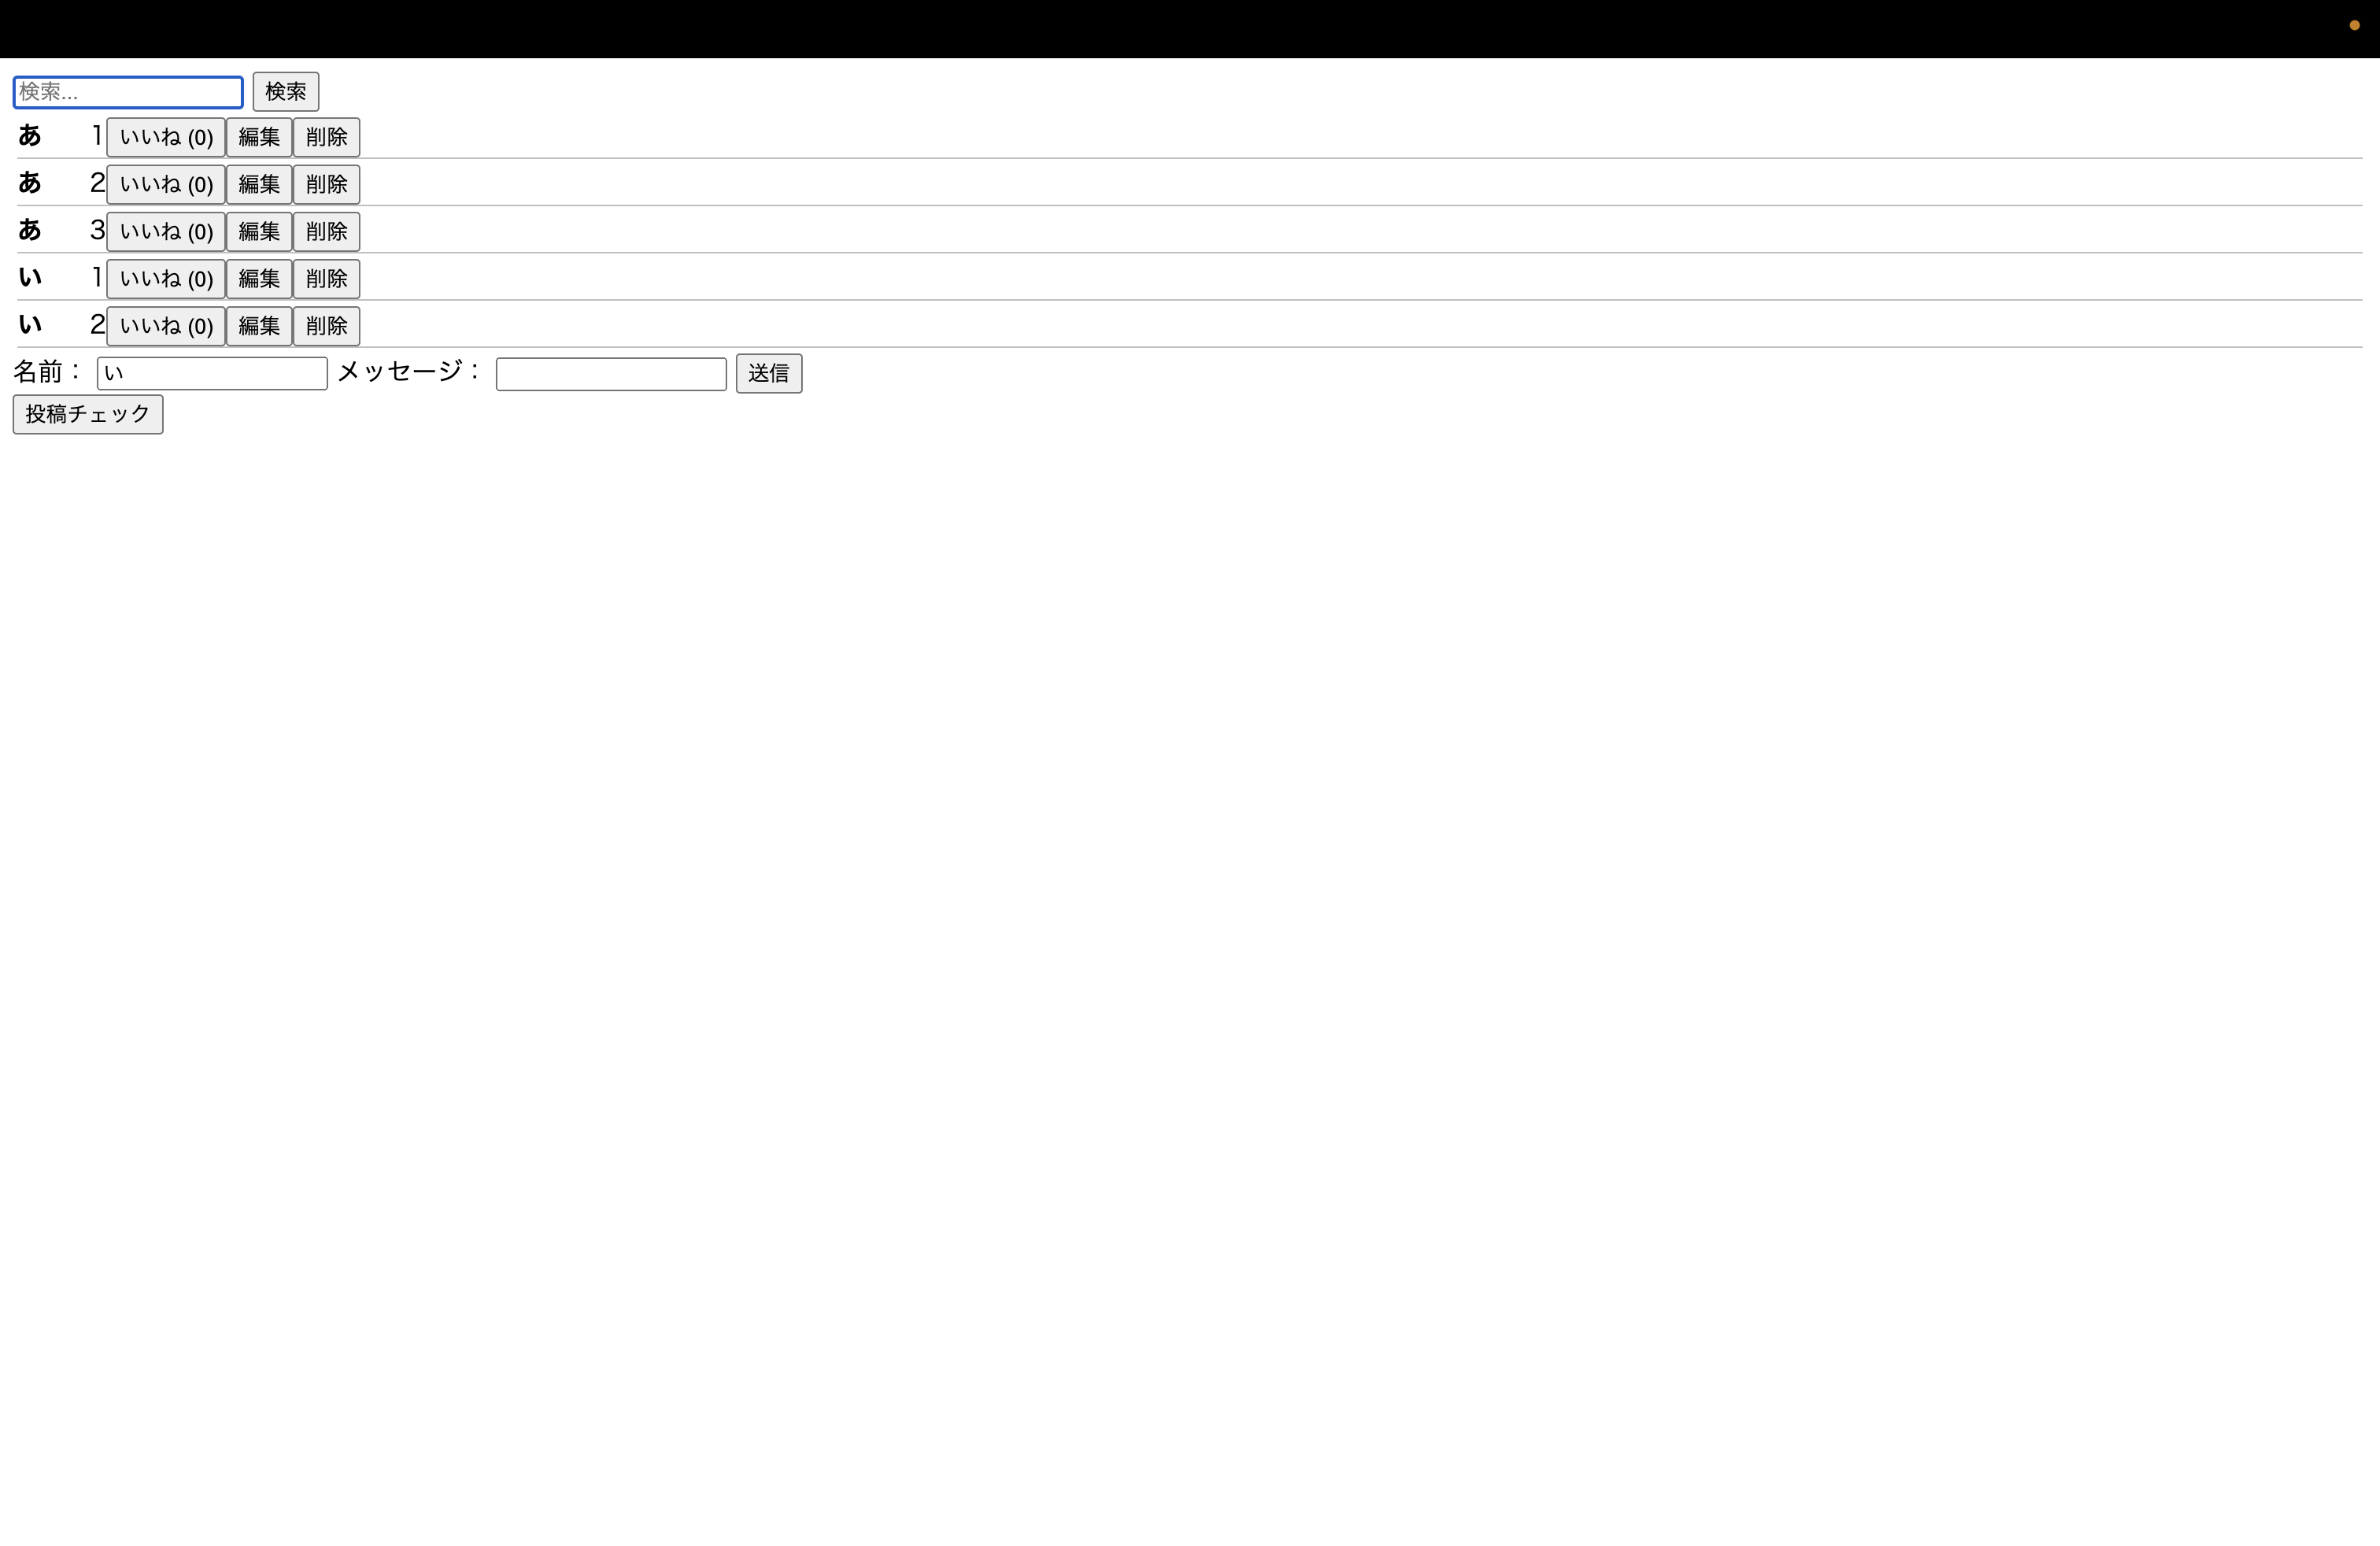
\includegraphics[width=15cm]{reiauto.png}
      \caption{画面のレイアウト}
      \label{reiauto}
\end{figure}

\end{document} 


\section{管理者向けの説明}
このサーバーを立ち上げる手順以下のようになる.
\begin{enumerate}
  \setlength{\leftskip}{0pt}
  \item[(1)]ターミナルを開き,node app8.js と入力(ホスト名はlocalhost,ポート番号は8080).

  \item[(2)]別のウィンドウでターミナルを開き,telnet localhost 8080 と入力.
  \item[(3)]WebブラウザのURL欄にhttp://localhost:8080/public/bbs.html と入力し,ページを表示する.
\end{enumerate}
